\section{Цель работы}

\begin{enumerate}
	\item Установить и настроить пакет GPG 2
	\item Создать набор ключей в Kleopatra
	\item Экспортировать свой ключ, импортировать ключ другого участника эксперимента
	\item Зашифровать файл и отправить другому человеку, расшифровать чужой файл
	\item Выполнить те же пункты, используя консольный интерфейс
\end{enumerate}

\section{Ход работы}

\subsection{Использование GPG с помощью интерфейса Kleopatra}

Установим необходимые инструменты:

\begin{verbatim}[language=bash,caption={Установка GPG}]
artyom@gpg:~$ sudo apt-get install kleopatra gnupg2
\end{verbatim}

Запустим Kleopatra. Перед нами появится главное окно:

\begin{figure}[H]
	\centering
	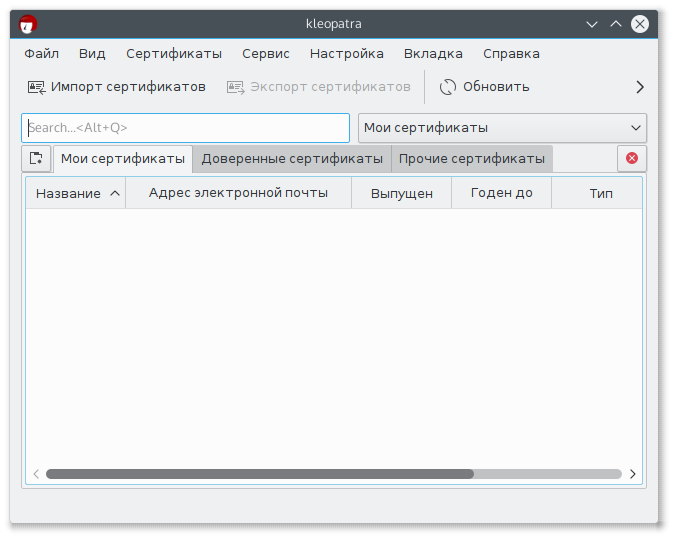
\includegraphics[width=0.8\textwidth]{figures/screen1.png}
	\caption{Главное окно программы Kleopatra}
\end{figure}

Через меню <<Файл>> запустим мастер создания ключа

\begin{figure}[H]
	\centering
	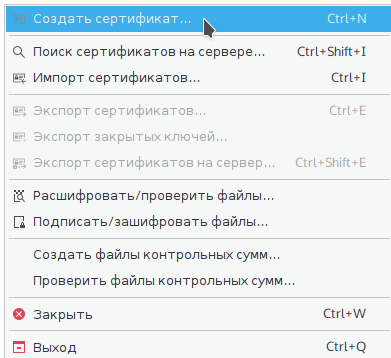
\includegraphics[width=0.7\textwidth]{figures/screen2.png}
	\caption{Меню <<Файл>>}
\end{figure}

В данной работе нас интересуют ключи PGP, поэтому выберем первый пункт.

\begin{figure}[H]
	\centering
	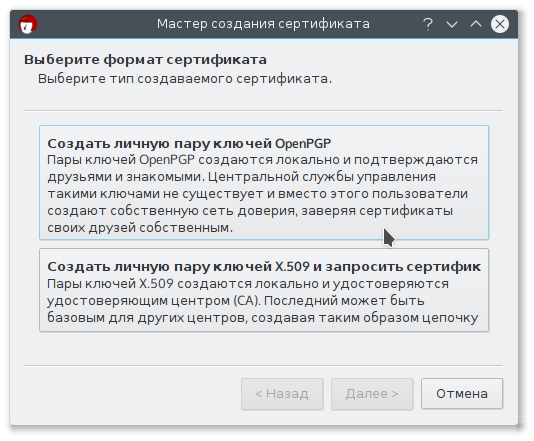
\includegraphics[width=0.8\textwidth]{figures/screen3.png}
	\caption{Создание ключа}
\end{figure}

Укажем свои реквизиты

\begin{figure}[H]
	\centering
	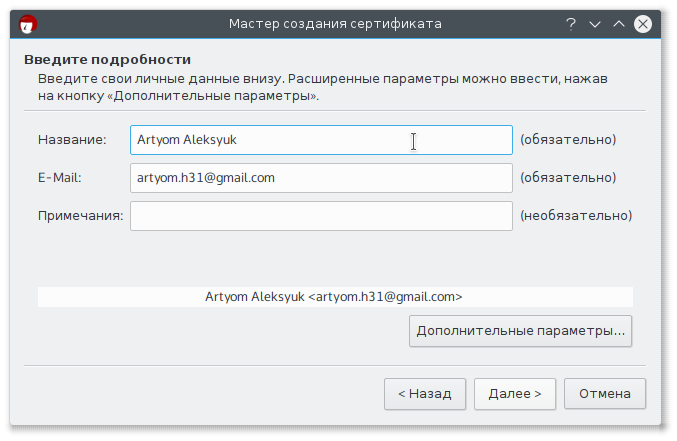
\includegraphics[width=0.8\textwidth]{figures/screen4.png}
	\caption{Создание ключа}
\end{figure}

В дополнительных параметрах проверим, что используются достаточная длина ключа, а также ограничим срок годности ключа.

\begin{figure}[H]
	\centering
	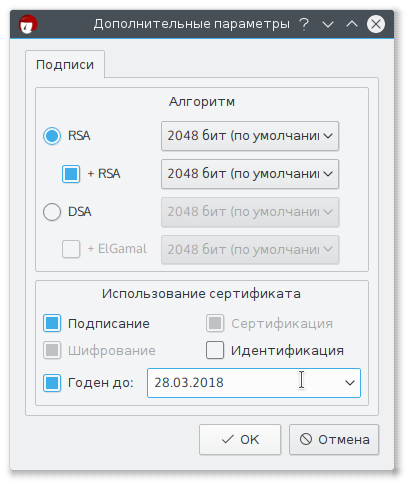
\includegraphics[width=0.6\textwidth]{figures/screen5.png}
	\caption{Создание ключа}
\end{figure}

Введем пароль

\begin{figure}[H]
	\centering
	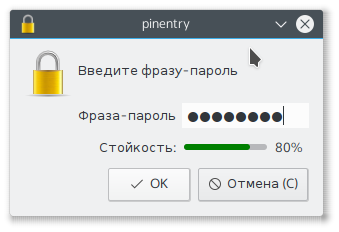
\includegraphics[width=0.5\textwidth]{figures/screen6.png}
	\caption{Создание ключа}
\end{figure}

Voilà!

\begin{figure}[H]
	\centering
	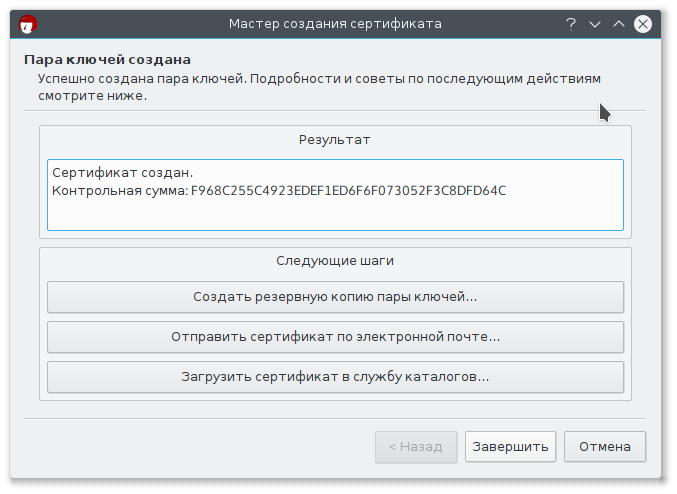
\includegraphics[width=0.8\textwidth]{figures/screen7.png}
	\caption{Создание ключа}
\end{figure}

Наш ключ появился в списке

\begin{figure}[H]
	\centering
	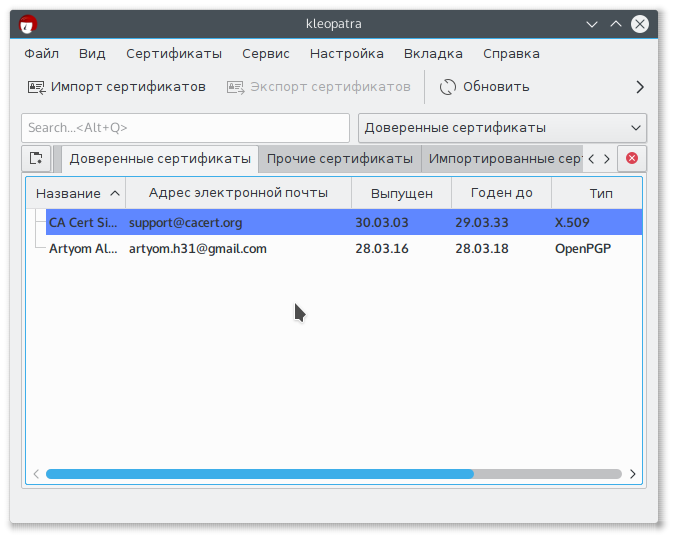
\includegraphics[width=0.8\textwidth]{figures/screen9.png}
	\caption{Ключи}
\end{figure}

Получим сертификат от другого участника эксперимента, импортируем его.

\begin{figure}[H]
	\centering
	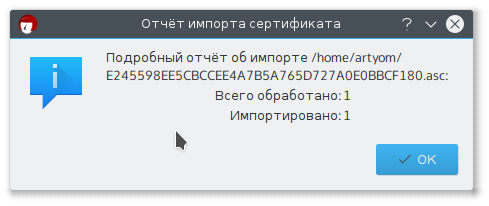
\includegraphics[width=0.8\textwidth]{figures/screen8.png}
	\caption{Импорт сертификата}
\end{figure}

Видим его в списке

\begin{figure}[H]
	\centering
	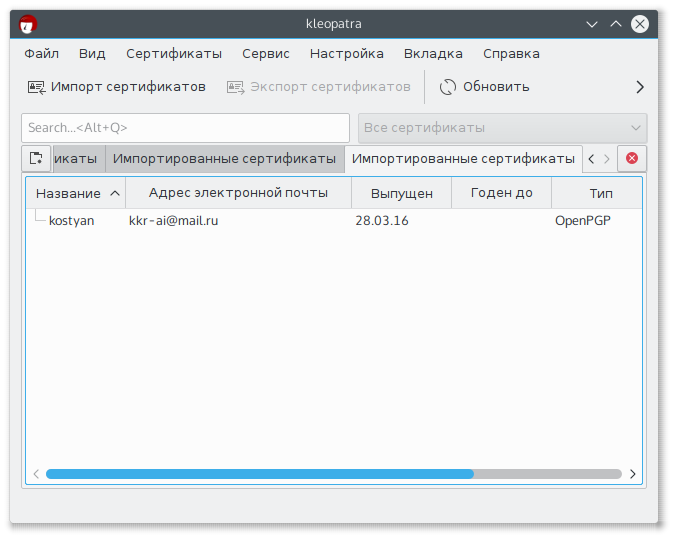
\includegraphics[width=0.8\textwidth]{figures/screen17.png}
	\caption{Сертификаты}
\end{figure}

Зашифруем файл. Для удобства обмена включим использование текстового представления зашифрованных данных.

\begin{figure}[H]
	\centering
	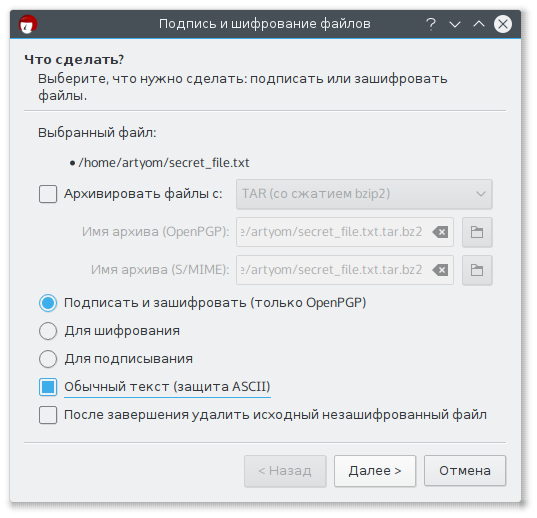
\includegraphics[width=0.8\textwidth]{figures/screen18.png}
	\caption{Шифрование}
\end{figure}

Выберем свой и чужой ключ

\begin{figure}[H]
	\centering
	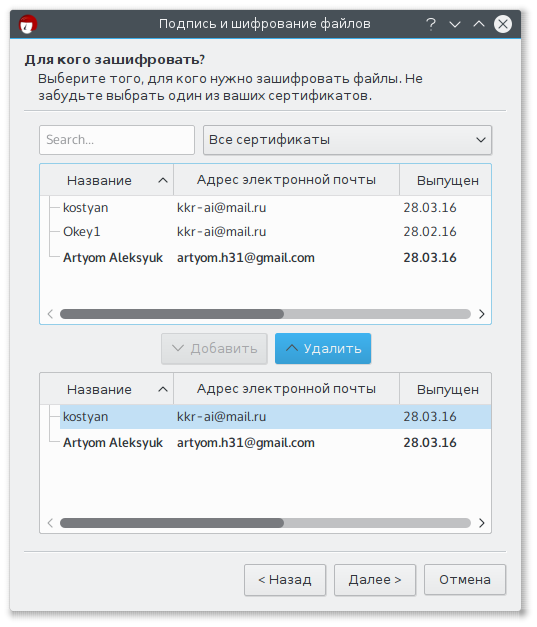
\includegraphics[width=0.8\textwidth]{figures/screen19.png}
	\caption{Шифрование}
\end{figure}

Выберем открытый ключ, с помощью которого будем шифровать

\begin{figure}[H]
	\centering
	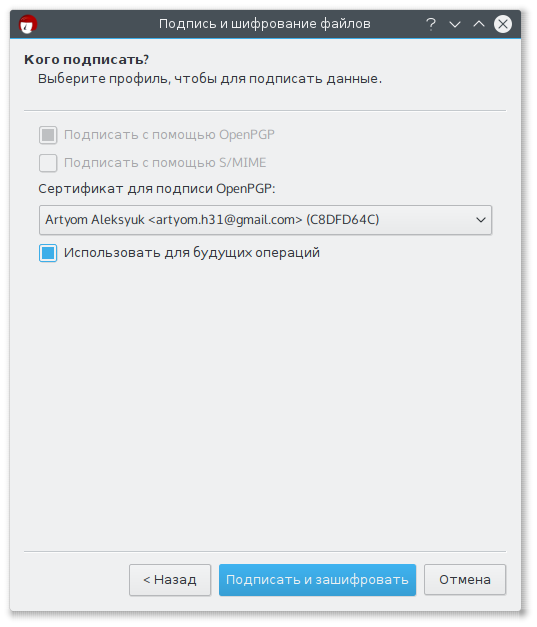
\includegraphics[width=0.8\textwidth]{figures/screen20.png}
	\caption{Шифрование}
\end{figure}

Сообщение об успехе

\begin{figure}[H]
	\centering
	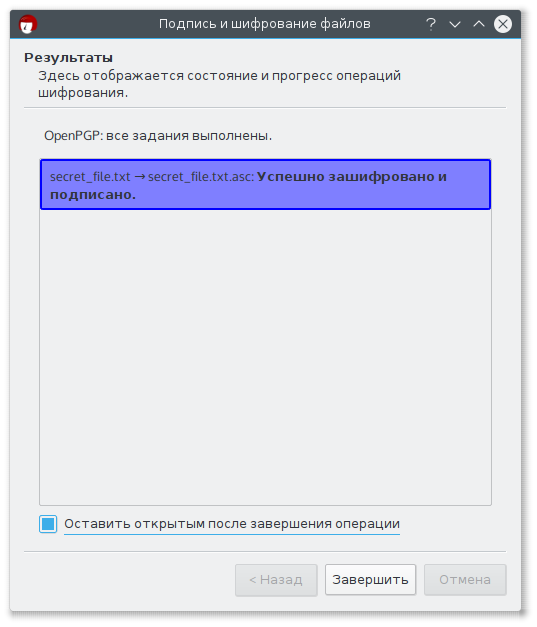
\includegraphics[width=0.8\textwidth]{figures/screen21.png}
	\caption{Шифрование}
\end{figure}

Так выглядит зашифрованный файл

\begin{figure}[H]
	\centering
	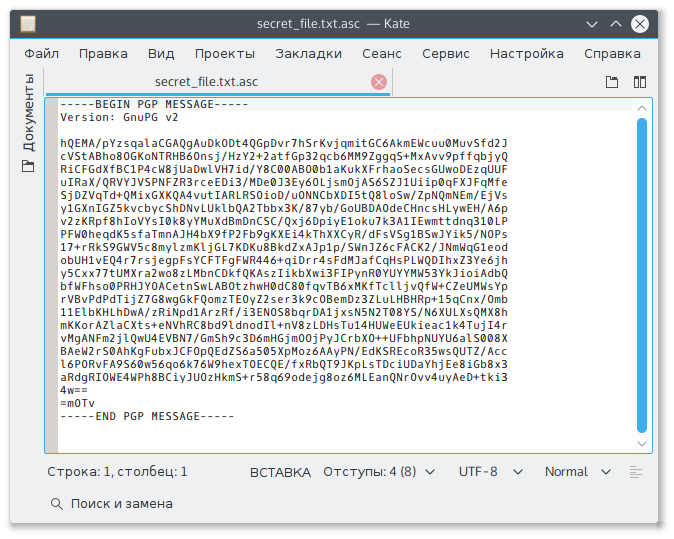
\includegraphics[width=0.8\textwidth]{figures/screen14.png}
	\caption{Зашифрованный файл}
\end{figure}

Теперь попробуем расшифровать файл, для этого запустим мастер из меню <<Файл>>.

\begin{figure}[H]
	\centering
	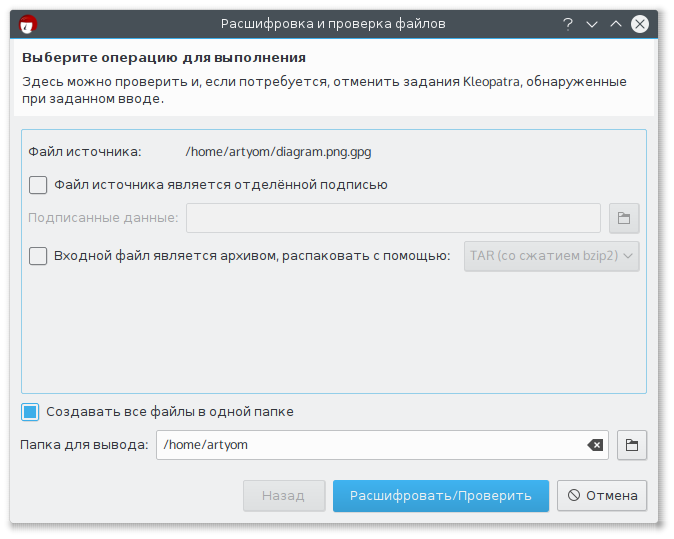
\includegraphics[width=0.8\textwidth]{figures/screen15.png}
	\caption{Расшифровка}
\end{figure}

Так быстро?

\begin{figure}[H]
	\centering
	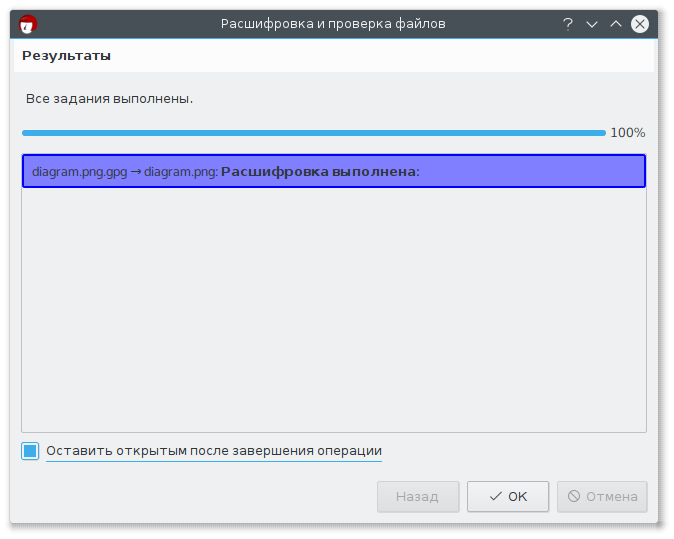
\includegraphics[width=0.8\textwidth]{figures/screen16.png}
	\caption{Расшифровка}
\end{figure}

Ниже представлено расшифрованное изображение

\begin{figure}[H]
	\centering
	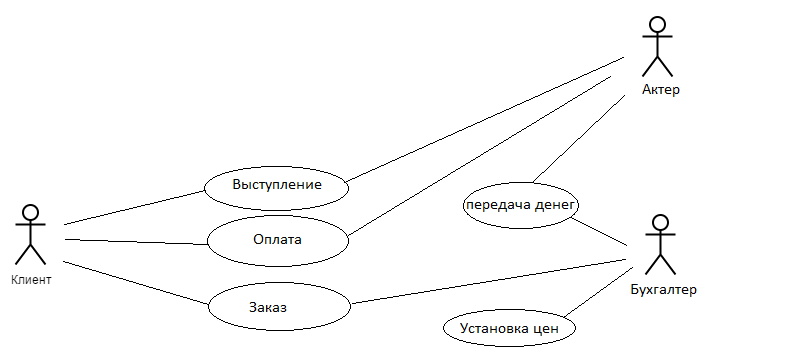
\includegraphics[width=0.8\textwidth]{figures/diagram.png}
	\caption{Расшифрованное изображение}
\end{figure}

\subsection{Использование GPG с помощью консольного интерфейса}

Эксперименты будут проводиться на другой машине. Попробуем вывести список ключей.

\begin{verbatim}  
artyom@artyom-H97-D3H:~/Projects/InfoSecCourse/gpg$ gpg2 --list-keys
\end{verbatim}

Пусто. Нужно создать новый ключ.

\begin{verbatim}
artyom@artyom-H97-D3H:~/Projects/InfoSecCourse/gpg$ gpg2 --gen-key
gpg (GnuPG) 2.0.28; Copyright (C) 2015 Free Software Foundation, Inc.
This is free software: you are free to change and redistribute it.
There is NO WARRANTY, to the extent permitted by law.

Выберите тип ключа:
(1) RSA и RSA (по умолчанию)
(2) DSA и Elgamal
(3) DSA (только для подписи)
(4) RSA (только для подписи)
Ваш выбор? 1
длина ключей RSA может быть от 1024 до 4096 бит.
Какой размер ключа Вам необходим? (2048) 
Запрошенный размер ключа - 2048 бит
Выберите срок действия ключа.
0 = без ограничения срока действия
<n>  = срок действия ключа - n дней
<n>w = срок действия ключа - n недель
<n>m = срок действия ключа - n месяцев
<n>y = срок действия ключа - n лет
Срок действия ключа? (0) 2y
Ключ действителен до Ср. 28 марта 2018 00:55:57 MSK
Все верно? (y/N) y

GnuPG необходимо составить ID пользователя в качестве идентификатора
 ключа.

Ваше настоящее имя: Artyom Aleksyuk
Адрес электронной почты: artyom.h31@gmail.com
Комментарий: 
Вы выбрали следующий ID пользователя:
"Artyom Aleksyuk <artyom.h31@gmail.com>"

Сменить (N)Имя, (C)Комментарий, (E)Адрес или (O)Принять/(Q)Выход? O
Для защиты закрытого ключа необходима фраза-пароль.


(process:22404): GLib-WARNING **: /build/glib2.0-MuyBSS/glib2.0-2.46.2/
./glib/gmem.c:482: custom memory allocation vtable not supported

(process:22412): GLib-WARNING **: /build/glib2.0-MuyBSS/glib2.0-2.46.2/
./glib/gmem.c:482: custom memory allocation vtable not supported
Необходимо получить много случайных чисел. Желательно, чтобы Вы
в процессе генерации выполняли какие-то другие действия (печать
на клавиатуре, движения мыши, обращения к дискам); это даст генератору
случайных чисел больше возможностей получить достаточное количество
 энтропии.
Необходимо получить много случайных чисел. Желательно, чтобы Вы
в процессе генерации выполняли какие-то другие действия (печать
на клавиатуре, движения мыши, обращения к дискам); это даст генератору
случайных чисел больше возможностей получить достаточное количество
 энтропии.
gpg: ключ 92682E10 помечен как абсолютно доверенный.
открытый и закрытый ключи созданы и подписаны.

gpg: проверка таблицы доверия
gpg: требуется 3 с ограниченным доверием, 1 с полным, модель доверия PGP
gpg: глубина: 0  верных:   1  подписанных:   0  доверие: 0-, 0q, 0n,
 0m, 0f, 1u
gpg: срок следующей проверки таблицы доверия 2018-03-27
pub   2048R/92682E10 2016-03-27 [годен до: 2018-03-27]
Отпечаток ключа = 3642 F44F 0375 4B21 A4A1  F188 2704 20BB 9268 2E10
uid     [абсолютное] Artyom Aleksyuk <artyom.h31@gmail.com>
sub   2048R/9AAC34E0 2016-03-27 [годен до: 2018-03-27]
artyom@artyom-H97-D3H:~/Projects/InfoSecCourse/gpg$ gpg2 --list-keys
/home/artyom/.gnupg/pubring.gpg
-------------------------------
pub   2048R/92682E10 2016-03-27 [годен до: 2018-03-27]
uid     [абсолютное] Artyom Aleksyuk <artyom.h31@gmail.com>
sub   2048R/9AAC34E0 2016-03-27 [годен до: 2018-03-27]
\end{verbatim}

В списке появился новый ключ:

\begin{verbatim}
artyom@artyom-H97-D3H:~/Projects/InfoSecCourse/gpg$ gpg2 --list-keys
/home/artyom/.gnupg/pubring.gpg
-------------------------------
pub   2048R/92682E10 2016-03-27 [годен до: 2018-03-27]
uid     [абсолютное] Artyom Aleksyuk <artyom.h31@gmail.com>
sub   2048R/9AAC34E0 2016-03-27 [годен до: 2018-03-27]
\end{verbatim}

Экспортируем его.

\begin{verbatim}
artyom@artyom-H97-D3H:~/Projects/InfoSecCourse/gpg$ gpg2 --export
 --armor 92682E10
-----BEGIN PGP PUBLIC KEY BLOCK-----
Version: GnuPG v2
...
\end{verbatim}

Попробуем зашифровать файл. Связь с другим участником эксперимента прервалась (вероятно, владельцы переданного ему секрета уже приехали за ним), поэтому в качестве получателя будет машина, на которая проводилась первая часть экспериментов.

Импортируем ключ:

\begin{verbatim}  
artyom@artyom-H97-D3H:~/Projects/InfoSecCourse/gpg$ gpg2
 --import ~/Downloads/F968C255C4923EDEF1ED6F6F073052F3C8DFD64C.asc 
gpg: ключ C8DFD64C: импортирован открытый ключ "Artyom Aleksyuk
 <artyom.h31@gmail.com>"
gpg: Всего обработано: 1
gpg:               импортировано: 1  (RSA: 1)
artyom@artyom-H97-D3H:~/Projects/InfoSecCourse/gpg$ gpg2 --list-keys
/home/artyom/.gnupg/pubring.gpg
-------------------------------
pub   2048R/92682E10 2016-03-27 [годен до: 2018-03-27]
uid     [абсолютное] Artyom Aleksyuk <artyom.h31@gmail.com>
sub   2048R/9AAC34E0 2016-03-27 [годен до: 2018-03-27]

pub   2048R/C8DFD64C 2016-03-27 [годен до: 2018-03-28]
uid     [неизвестно] Artyom Aleksyuk <artyom.h31@gmail.com>
sub   2048R/72C1CBCB 2016-03-27 [годен до: 2018-03-28]
\end{verbatim}

Запустим шифрование:

\begin{verbatim}
artyom@artyom-H97-D3H:~/Projects/InfoSecCourse/gpg$ gpg2 --armor
 --encrypt secret.txt 
Не задан ID пользователя (можно использовать "-r").

Текущие получатели:

Введите ID пользователя. Пустая строка для завершения: C8DFD64C
gpg: 72C1CBCB: Нет свидетельств того, что данный ключ принадлежит
 названному пользователю

pub  2048R/72C1CBCB 2016-03-27 Artyom Aleksyuk <artyom.h31@gmail.com>
Отпечаток главного ключа: F968 C255 C492 3EDE F1ED  6F6F 0730 52F3
 C8DF D64C
Отпечаток подключа: 93B0 41C2 D4F3 17DC 0E25  3252 9D78 21E7 72C1 CBCB

Нет уверенности в том, что ключ принадлежит человеку, указанному
в ID пользователя ключа. Если Вы ТОЧНО знаете, что делаете,
можете ответить на следующий вопрос утвердительно.

Все равно использовать данный ключ? (y/N) y

Текущие получатели:
2048R/72C1CBCB 2016-03-27 "Artyom Aleksyuk <artyom.h31@gmail.com>"

Введите ID пользователя. Пустая строка для завершения: 
\end{verbatim}

В директории появился новый файл

\begin{verbatim}
artyom@artyom-H97-D3H:~/Projects/InfoSecCourse/gpg$ ls
log.txt  report.tex  secret.txt  secret.txt.asc
\end{verbatim}

Импортируем открытый ключ на другой машине

\begin{figure}[H]
	\centering
	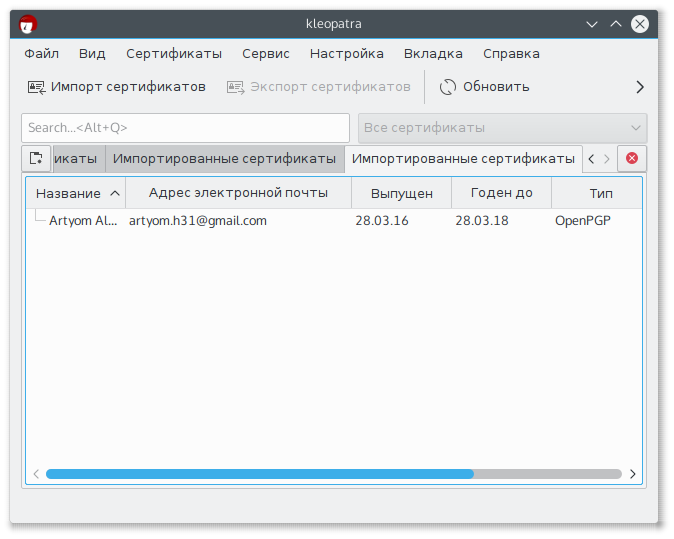
\includegraphics[width=0.8\textwidth]{figures/screen22.png}
	\caption{Импорт ключа}
\end{figure}

Запустим расшифровку

\begin{figure}[H]
	\centering
	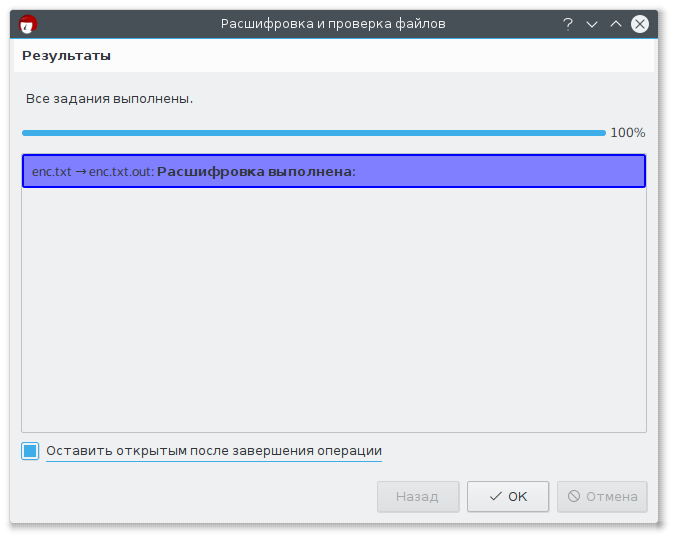
\includegraphics[width=0.8\textwidth]{figures/screen23.png}
	\caption{Расшифровка}
\end{figure}

Проверим, что файл успешно расшифрован:

\begin{verbatim}
artyom@gpg:~$ cat enc.txt.out 
Do you really expect to find a secret here?
\end{verbatim}